\documentclass{beamer}
\usepackage{boondox-calo} % lowercase calligraphic letters
\usepackage[backend=biber]{biblatex}

\beamertemplatenavigationsymbolsempty
\usetheme{Warsaw}
\addbibresource{reference.bib}
\setbeamertemplate{bibliography item}{\insertbiblabel}

\newcommand
{\const}
[1]
{\mathfrak{#1}}

\title{Multiconnectivity Based Joint Scheduling of URLLC and eMBB Traffic in 5G Networks}
\author{Tran Phong Binh}
\institute{Department of Computer Science, National Tsing Hua University}
\date{\today}

\begin{document}

\begin{frame}
  \titlepage
\end{frame}

\begin{frame}
  \frametitle{Scenario 2: Neighborhood}
  \begin{itemize}
    \item There are 2,000 households (up to 8,000 eMBB users e.g. downloading files, watching YouTube, surfing Facebook/Instagramm, etc.)
    \item During work hours and at night, there are only a few URLLC autonomous cars moving around
    \item Downlink transmission accounts for eMBB users' requests and URLLC autonomous cars' controlling
    \item Uplink transmission (whose bandwidth is separated from that of downlink) is responsible for uploading cars' data (e.g. camera images, GPS, sensors data, etc.) to server for navigation processing
  \end{itemize}
\end{frame}

\begin{frame}
  \frametitle{Scenario 3: Hotel}
  \begin{itemize}
    \item There are 10 rooms (up to 40 eMBB users) in a floor
    \item There are 2 URLLC service robots delivering food and miscellaneous items
    \item Downlink transmission accounts for eMBB users' requests and URLLC service robots' controlling
    \item Uplink transmission (whose bandwidth is separated from that of downlink) is responsible for uploading robots' data (i.e. camera images, sensors data, etc.) to server for navigation processing
  \end{itemize}
\end{frame}

\begin{frame}
  \frametitle{Problem Statement}
  \begin{itemize}
    \item Downlink transmission is considered
    \item Problems:
      \begin{itemize}
        \item One base station cannot serve that many eMBB users due to bandwidth limitation
        \item eMBB users located at base stations' coverage edges suffer from poor capacity due to path loss, channel fading, and shadowing (especially if mmWave is employed)
      \end{itemize}
    \item Solution: Multiconnectivity
    \item Motivation:
    \item Pros and Cons:
      \begin{itemize}
        \item (+) Resolves the aforementioned issues
        \item (-) Interference among base stations needs to be addressed
        \item (-) Requires eMBB user equipments to support MIMO (Multiple-Input and Multiple-Output)
      \end{itemize}
  \end{itemize}
\end{frame}

\begin{frame}
  \frametitle{eMBB \& URLLC Interference Problem of Multiconnectivity}
  \begin{itemize}
    \item eMBB interference problem: Even without taking URLLC user equipments into account, interference may occur among eMBB user equipments of \emph{different} base stations
    \item URLLC interference problem:
      \begin{itemize}
        \item If for each base station, the same dedicated channel is allocated for URLLC traffic, then interference may occur among URLLC user equipments of \emph{different} base stations
        \item If for all base stations, mutually exclusive dedicated channels are allocated for URLLC traffic, then interference may occur between URLLC user equipments of one base station and eMBB user equipments of others
        \item If URLLC puncture system is used on all base stations, then interference may occur between URLLC user equipments of one base station and eMBB/URLLC user equipments of others
      \end{itemize}
  \end{itemize}
\end{frame}

\begin{frame}
  \frametitle{eMBB \& URLLC Interference Problem of Multiconnectivity}
  \begin{itemize}
    \item Solution 1: Mathematical optimization with optimal analysis (currently researching \cite{dualConnectivityOptimal})
    \item Solution 2: Approximation algorithm with approximation ratio analysis (currently researching \cite{dualConnectivityApproximate})
  \end{itemize}
\end{frame}

\begin{frame}
  \frametitle{eMBB \& URLLC Interference Problem of Multiconnectivity}
  \begin{itemize}
    \item Solution 3: W-CDMA (Wideband Code Division Multiple Access)
    \item Motivation: LEACH (Low-Energy Adaptive Clustering Hierarchy)
    \item Pros and Cons:
      \begin{itemize}
        \item (+) Preserves the full spectral resource
        \item (+) Fits with the often small number of base stations
        \item (+) Simplifies the mathematical model of the system
        \item (-) Introduces redundant bits
        \item (-) Requires eMBB user equipments to support \emph{multiple} CDMA
        \item (-) Requires URLLC user equipments to support CDMA
      \end{itemize}
    \item However, the number of redundant bits required is the number of orthogonal basis to assign to each base station i.e. the number of base stations, which is negligible
    \item On the other hand, it is projected that devices are becoming more and more advanced, so expecting user equipments to support multiple CDMA at the same time is plausible
  \end{itemize}
\end{frame}

\begin{frame}
  \frametitle{Spectral Utilization Problem of Dedicated URLLC Channel}
  \begin{itemize}
    \item If a bandwidth $\const{w}$ is dedicated to serve URLLC requests, a total of $\const{w} \times \const{b}$ bandwidth is wasted, where $\const{b}$ is the number of base stations
    \item Solution: URLLC superposition/puncturing
    \item Motivation:
    \item Pros and Cons:
  \end{itemize}
\end{frame}

\begin{frame}
  \frametitle{System Model}
  \begin{figure}
    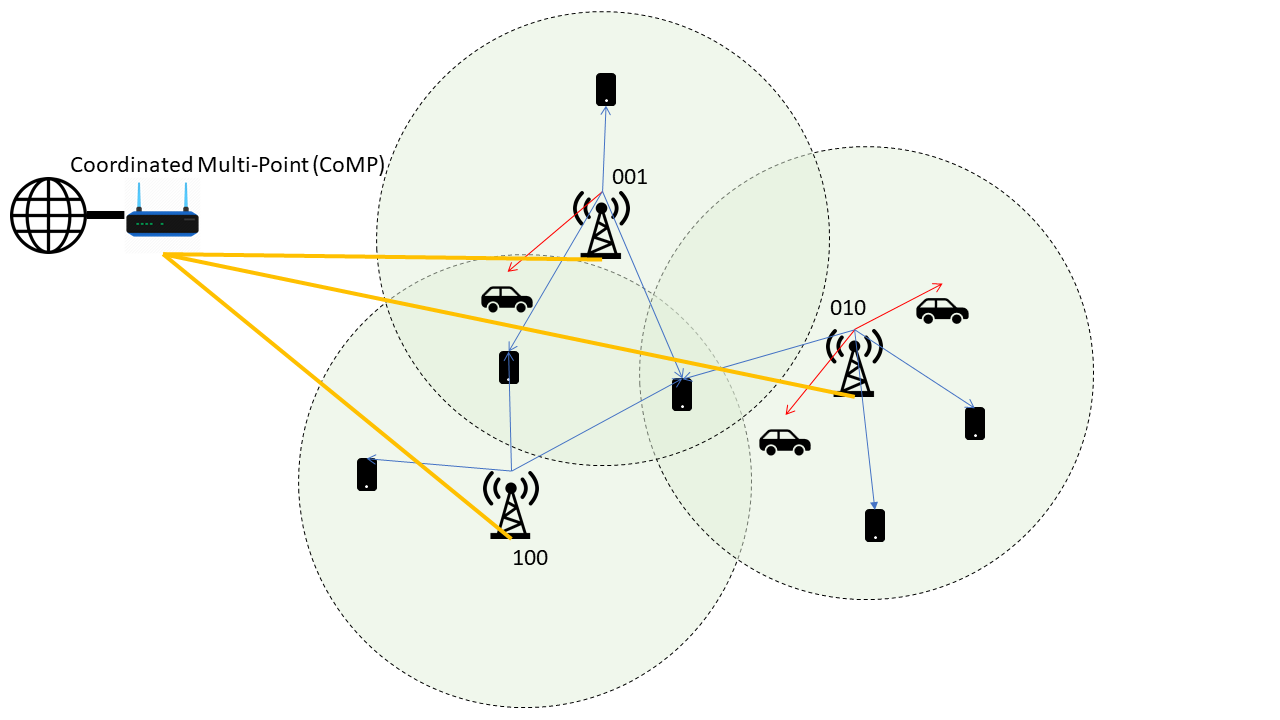
\includegraphics[width=\textwidth]{system_model}
    \caption{System model}
  \end{figure}
\end{frame}

\begin{frame}
  \frametitle{System Framework}
  \begin{figure}
    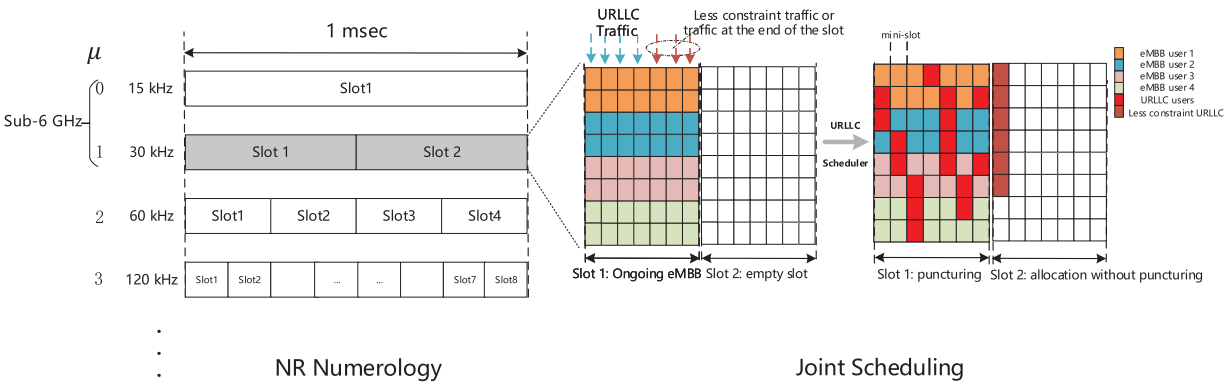
\includegraphics[width=\textwidth]{system_framework}
    \caption{System framework}
  \end{figure}
\end{frame}

\begin{frame}
  \frametitle{References}
  \printbibliography[heading=none]
\end{frame}

\end{document}
